\documentclass[border=0.2cm]{standalone}

\usepackage{tikz}
\usetikzlibrary{shapes.geometric, shapes.misc}
\usetikzlibrary{cd, fit, calc}
\usetikzlibrary{positioning}
\usetikzlibrary{decorations.markings, decorations.pathreplacing}
\usepackage{medl_colors}
\usepackage{ifthen}

\graphicspath{ {./images/} }

\newcommand{\customArrow}[5]{
    \ifthenelse{\equal{#5}{right}}{%
         \draw[dashed, bthickline] (#1,#2) -- (#3-1,#4);
         \draw[-Triangle, bthickline] (#3-0.9,#4) -- (#3,#4) {};
    }{%
         \draw[dashed, bthickline] (#1,#2) -- (#3+1,#4);
         \draw[-Triangle, bthickline] (#3+0.9,#4) -- (#3,#4) {};
    }
}

\begin{document}
\begin{tikzpicture}


\node[scale = .4] (pica) at (0,0){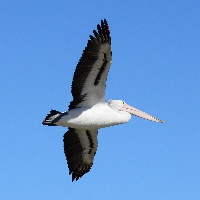
\includegraphics {images/noisy_image_00.jpg}};
\node[right of=pica, scale = .4, node distance=4cm] (picb) 
{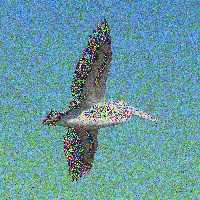
\includegraphics {images/noisy_image_03.jpg}};
\node[right of=picb, scale = .4, node distance=5cm] (picd) {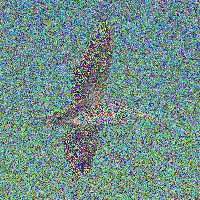
\includegraphics {images/noisy_image_06.jpg}};
\node[right of=picd, scale = .4, node distance=4cm] (pice) {
\includegraphics {images/noisy_image_10.jpg}};

\draw [-Triangle, bthickline] ($(pica.east)+(0,1)$) -- ($(picb.west)+(0,1)$) node [above, midway] (ab1) {};
\draw [-Triangle, bthickline] ($(picb.west)+(0,-1)$) -- ($(pica.east)+(0,-1)$) node [above, midway] (ab2) {};
\customArrow{5.4}{1}{7.6}{1}{right};
\customArrow{7.6}{-1}{5.4}{-1}{left};

\draw [-Triangle, bthickline] ($(picd.east)+(0,1)$) -- ($(pice.west)+(0,1)$) node[above, midway](de1){};
\draw [-Triangle, bthickline] ($(pice.west)+(0,-1)$) -- ($(picd.east)+(0,-1)$) node[above, midway](de2){};
\draw [-Triangle, bthickline] ($(picb.north)+(0,0.5)$) -- ($(picd.north)+
(0,0.5)$) node[above, midway](de3){\LARGE {Encoder}};
\draw [-Triangle, bthickline] ($(picd.south)+(0,-0.5)$) -- ($(picb.south)+
(0,-0.5)$) node[below, midway](de3){\LARGE {Decoder}};

\end{tikzpicture}
\end{document}